\documentclass{beamer}
\usepackage{../../shared/styles/custom}
% =============================================================================
% ML TEACHING MATHEMATICAL NOTATION CONVENTIONS
% =============================================================================
% Based on standard ML textbooks: Murphy's "Machine Learning: A Probabilistic Perspective",
% Bishop's "Pattern Recognition and Machine Learning", and "Mathematics for Machine Learning"

% =============================================================================
% CORE NOTATION STANDARDS
% =============================================================================

% SCALARS: Regular italics (lowercase for variables, uppercase for constants)
% Examples: x, y, n, d, k, \theta, \alpha, \lambda, \sigma

% VECTORS: Bold lowercase letters
% Examples: \mathbf{x}, \mathbf{w}, \mathbf{\mu}, \mathbf{\theta}

% MATRICES: Bold uppercase letters
% Examples: \mathbf{X}, \mathbf{W}, \mathbf{\Sigma}, \mathbf{\Lambda}

% SETS: Calligraphic uppercase
% Examples: \mathcal{D}, \mathcal{X}, \mathcal{Y}

% SPACES: Blackboard bold
% Examples: \mathbb{R}, \mathbb{Z}, \mathbb{N}

% =============================================================================
% VECTOR NOTATION (bold lowercase)
% =============================================================================

\newcommand{\vx}{\mathbf{x}}        % Input vector
\newcommand{\vy}{\mathbf{y}}        % Output vector
\newcommand{\vw}{\mathbf{w}}        % Weight vector
\newcommand{\vb}{\mathbf{b}}        % Bias vector
\newcommand{\vh}{\mathbf{h}}        % Hidden vector
\newcommand{\vz}{\mathbf{z}}        % Latent vector
\newcommand{\vf}{\mathbf{f}}        % Function vector
\newcommand{\vg}{\mathbf{g}}        % Gradient vector
\newcommand{\vu}{\mathbf{u}}        % Generic vector u
\newcommand{\vv}{\mathbf{v}}        % Generic vector v
\newcommand{\vzero}{\mathbf{0}}     % Zero vector
\newcommand{\vone}{\mathbf{1}}      % Ones vector

% Greek vectors (bold)
\newcommand{\vmu}{\boldsymbol{\mu}}     % Mean vector
\newcommand{\vtheta}{\boldsymbol{\theta}} % Parameter vector
\newcommand{\vlambda}{\boldsymbol{\lambda}} % Lambda vector
\newcommand{\valpha}{\boldsymbol{\alpha}}   % Alpha vector
\newcommand{\vbeta}{\boldsymbol{\beta}}     % Beta vector
\newcommand{\vxi}{\boldsymbol{\xi}}         % Xi vector
\newcommand{\vepsilon}{\boldsymbol{\epsilon}} % Epsilon vector

% =============================================================================
% MATRIX NOTATION (bold uppercase)
% =============================================================================

\newcommand{\mX}{\mathbf{X}}        % Data matrix
\newcommand{\mY}{\mathbf{Y}}        % Target matrix
\newcommand{\mW}{\mathbf{W}}        % Weight matrix
\newcommand{\mA}{\mathbf{A}}        % Generic matrix A
\newcommand{\mB}{\mathbf{B}}        % Generic matrix B
\newcommand{\mC}{\mathbf{C}}        % Generic matrix C
\newcommand{\mH}{\mathbf{H}}        % Hidden layer matrix / Hessian
\newcommand{\mI}{\mathbf{I}}        % Identity matrix
\newcommand{\mJ}{\mathbf{J}}        % Jacobian matrix
\newcommand{\mK}{\mathbf{K}}        % Kernel matrix
\newcommand{\mL}{\mathbf{L}}        % Loss matrix / Cholesky factor
\newcommand{\mP}{\mathbf{P}}        % Projection matrix
\newcommand{\mQ}{\mathbf{Q}}        % Orthogonal matrix
\newcommand{\mR}{\mathbf{R}}        % Rotation matrix
\newcommand{\mS}{\mathbf{S}}        % Scatter matrix
\newcommand{\mU}{\mathbf{U}}        % Left singular vectors
\newcommand{\mV}{\mathbf{V}}        % Right singular vectors

% Greek matrices (bold)
\newcommand{\mSigma}{\boldsymbol{\Sigma}}   % Covariance matrix
\newcommand{\mLambda}{\boldsymbol{\Lambda}} % Diagonal eigenvalue matrix
\newcommand{\mPhi}{\boldsymbol{\Phi}}       % Feature matrix
\newcommand{\mPsi}{\boldsymbol{\Psi}}       % Basis matrix
\newcommand{\mTheta}{\boldsymbol{\Theta}}   % Parameter matrix

% =============================================================================
% SETS AND SPACES (following Bishop/Murphy conventions)
% =============================================================================

\newcommand{\cD}{\mathcal{D}}       % Dataset
\newcommand{\cH}{\mathcal{H}}       % Hypothesis space
\newcommand{\cX}{\mathcal{X}}       % Input space
\newcommand{\cY}{\mathcal{Y}}       % Output space
\newcommand{\cF}{\mathcal{F}}       % Function space
\newcommand{\cG}{\mathcal{G}}       % Gaussian process
\newcommand{\cL}{\mathcal{L}}       % Lagrangian / Loss
\newcommand{\cN}{\mathcal{N}}       % Normal distribution
\newcommand{\cU}{\mathcal{U}}       % Uniform distribution
\newcommand{\cB}{\mathcal{B}}       % Bernoulli distribution
\newcommand{\cP}{\mathcal{P}}       % Probability distribution

% Number systems
\newcommand{\Real}{\mathbb{R}}      % Real numbers
\newcommand{\Nat}{\mathbb{N}}       % Natural numbers
\newcommand{\Int}{\mathbb{Z}}       % Integers
\newcommand{\Complex}{\mathbb{C}}   % Complex numbers

% =============================================================================
% OPERATORS AND FUNCTIONS (following standard conventions)
% =============================================================================

% Prediction notation (commonly used in ML)
\newcommand{\yhat}{\hat{\vy}}        % Predicted output vector (bold)
\newcommand{\yhati}{\hat{y}_i}       % Predicted output for sample i (scalar)

% Common ML functions (with conflict resolution)
\providecommand{\sigmoid}{}
\renewcommand{\sigmoid}{\operatorname{sigmoid}}
\providecommand{\softmax}{}
\renewcommand{\softmax}{\operatorname{softmax}}
\providecommand{\ReLU}{}
\renewcommand{\ReLU}{\operatorname{ReLU}}
\providecommand{\sign}{}
\renewcommand{\sign}{\operatorname{sign}}
\DeclareMathOperator{\Gain}{Gain}    % Information gain
\DeclareMathOperator{\Entropy}{Entropy}
% KL divergence (check for conflicts)
\providecommand{\KL}{}
\renewcommand{\KL}{\operatorname{KL}}
\DeclareMathOperator{\MSE}{MSE}      % Mean squared error
\DeclareMathOperator{\MAE}{MAE}      % Mean absolute error
\DeclareMathOperator{\RMSE}{RMSE}    % Root mean squared error

% Classification metrics (upright text)
\newcommand{\TP}{\text{TP}}          % True positives
\newcommand{\TN}{\text{TN}}          % True negatives  
\newcommand{\FP}{\text{FP}}          % False positives
\newcommand{\FN}{\text{FN}}          % False negatives
\DeclareMathOperator{\Precision}{Precision}
\DeclareMathOperator{\Recall}{Recall}
\DeclareMathOperator{\Accuracy}{Accuracy}

% Transpose and inverse
\newcommand{\tp}{^\top}             % Transpose (Bishop/Murphy style)
\newcommand{\inv}{^{-1}}            % Matrix inverse
\newcommand{\pinv}{^{\dagger}}      % Pseudoinverse

% Norms (consistent with Murphy/Bishop)
\newcommand{\norm}[1]{\|#1\|}       % Generic norm
\newcommand{\normone}[1]{\|#1\|_1}  % L1 norm
\newcommand{\normtwo}[1]{\|#1\|_2}  % L2 norm
\newcommand{\norminf}[1]{\|#1\|_\infty} % L-infinity norm
\newcommand{\normF}[1]{\|#1\|_F}    % Frobenius norm

% Optimization operators (upright as in Murphy)
\providecommand{\argmin}{}
\renewcommand{\argmin}{\operatorname*{arg\,min}}
\providecommand{\argmax}{}
\renewcommand{\argmax}{\operatorname*{arg\,max}}
\DeclareMathOperator{\minimize}{minimize}
\DeclareMathOperator{\maximize}{maximize}
\DeclareMathOperator{\subjectto}{subject\,to}

% Matrix operations (upright) - use conditional definitions
\providecommand{\tr}{}
\renewcommand{\tr}{\operatorname{tr}}       % Trace
\providecommand{\det}{}
\renewcommand{\det}{\operatorname{det}}     % Determinant
\providecommand{\rank}{}
\renewcommand{\rank}{\operatorname{rank}}   % Rank
\providecommand{\span}{}
\renewcommand{\span}{\operatorname{span}}   % Span
\providecommand{\null}{}
\renewcommand{\null}{\operatorname{null}}   % Null space
\DeclareMathOperator{\range}{range} % Range/column space
\providecommand{\diag}{}
\renewcommand{\diag}{\operatorname{diag}}   % Diagonal operator
\providecommand{\vec}{}
\renewcommand{\vec}{\operatorname{vec}}     % Vectorization operator

% Probability and statistics (Murphy/Bishop style)
\newcommand{\Prob}{\mathbb{P}}      % Probability measure
\newcommand{\Exp}{\mathbb{E}}       % Expectation
\DeclareMathOperator{\Var}{Var}     % Variance
\DeclareMathOperator{\Cov}{Cov}     % Covariance
\DeclareMathOperator{\Corr}{Corr}   % Correlation
% KL divergence already defined above
\DeclareMathOperator{\MI}{I}        % Mutual information

% Activation functions (already defined above with conflict resolution)

% =============================================================================
% STANDARD PARAMETER CONVENTIONS (Murphy/Bishop style)
% =============================================================================

% Primary parameters: θ (theta) - following Murphy's convention
% Learning rates: α, η (alpha, eta)
% Regularization: λ (lambda)
% Precision: β (beta) - following Bishop
% Variance: σ² (sigma squared)
% Standard deviation: σ (sigma)
% Mean: μ (mu)

% Common scalars:
% n - number of training examples
% d - dimensionality of input
% k - number of classes/clusters
% m - number of hidden units
% T - number of time steps
% i, j - indices

% =============================================================================
% STANDARD NOTATION EXAMPLES (Murphy/Bishop style)
% =============================================================================

% Linear regression:      y = \vw\tp\vx + b
% Matrix form:            \vy = \mX\vw + b\vone
% Logistic regression:    p(y=1|\vx) = \sigmoid(\vw\tp\vx)
% Gaussian:               \vx \sim \cN(\vmu, \mSigma)
% Parameter update:       \vtheta_{t+1} = \vtheta_t - \alpha \nabla \cL(\vtheta_t)
% Likelihood:             p(\cD|\vtheta) = \prod_{i=1}^n p(y_i|\vx_i, \vtheta)
% Posterior:              p(\vtheta|\cD) \propto p(\cD|\vtheta)p(\vtheta)
% Prediction:             p(y^*|\vx^*, \cD) = \int p(y^*|\vx^*, \vtheta)p(\vtheta|\cD)d\vtheta

% =============================================================================
% COMMON MISTAKES TO AVOID
% =============================================================================

% ❌ WRONG NOTATION          →  ✅ CORRECT NOTATION (Murphy/Bishop style)

% Transpose:
% ❌ x^t, X^t              →  ✅ \vx\tp, \mX\tp
% ❌ x', X'                →  ✅ \vx\tp, \mX\tp

% Vectors vs Matrices vs Scalars:
% ❌ X (for vector)        →  ✅ \vx (bold lowercase)
% ❌ w (for weight vector) →  ✅ \vw (bold lowercase)
% ❌ x (for data matrix)   →  ✅ \mX (bold uppercase)
% ❌ \mathbf{\theta}       →  ✅ \vtheta (Greek vectors are bold)
% ❌ \mathbf{n}            →  ✅ n (scalars are not bold)

% Sets and distributions:
% ❌ R                     →  ✅ \Real (blackboard bold for number systems)
% ❌ \mathcal{R}           →  ✅ \Real (use blackboard for reals)
% ❌ Normal               →  ✅ \cN (calligraphic for distributions)

% Functions and operators:
% ❌ argmax                →  ✅ \argmax (upright operator)
% ❌ E[X]                  →  ✅ \Exp[X] (blackboard E for expectation)
% ❌ trace(A)              →  ✅ \tr(\mA) (upright operator)

% =============================================================================
% ALGORITHM NAME CONVENTIONS
% =============================================================================

% Use standard capitalizations as in textbooks:
% k-NN, SVM, PCA, GMM, EM, MAP, ML, SGD, Adam, RMSprop
% ReLU, tanh, sigmoid, softmax

\endinput

\usepackage{grffile}
%\beamerdefaultoverlayspecification{<+->}

\title{Lasso Regression}
\date{\today}
\author{Nipun Batra}
\institute{IIT Gandhinagar}
\begin{document}
  \maketitle
  
  
  
  
% \section{Linear Regression}

\begin{frame}{Lasso Regression}
\begin{itemize}[<+->]
	
	
	\item LASSO $\longrightarrow$ Least absolute shrinkage and selection operator
	\item Popular as it leads to a sparse solution.
	
\end{itemize}
\end{frame}

\begin{frame}{Constructing the Objective Function}
\begin{itemize}[<+->]

\item Find a $\vtheta_{\text{opt}}$ such that  \begin{equation}    \vtheta_{\text{opt}} =  \argmin_{\vtheta} {(\vy-\mX\vtheta)^T(\vy-\mX\vtheta)} : \ ||\vtheta||_1<s \end{equation}
\item Using KKT conditions
\begin{equation}
    \vtheta_{\text{opt}} = \underbrace{\argmin_{\vtheta}{(\vy-\mX\vtheta)^T(\vy-\mX\vtheta) + \delta^2||\vtheta||_1}}_\text{convex function}
\end{equation}
	
\end{itemize}


\end{frame}

\begin{frame}{Solving the Objective}
\begin{itemize}[<+->]

\item Since $||\vtheta||_1$ is not differentiable, we cannot solve,  \begin{equation}    \frac{\partial {(\vy-\mX\vtheta)^T(\vy-\mX\vtheta) + \delta^2||\vtheta||_1}}{\partial \vtheta} = 0 \end{equation}

\item How to Solve?
Use coordinate descent!
\end{itemize}

\end{frame}

\begin{frame}{Sample Dataset}

\begin{figure}
    \centering
    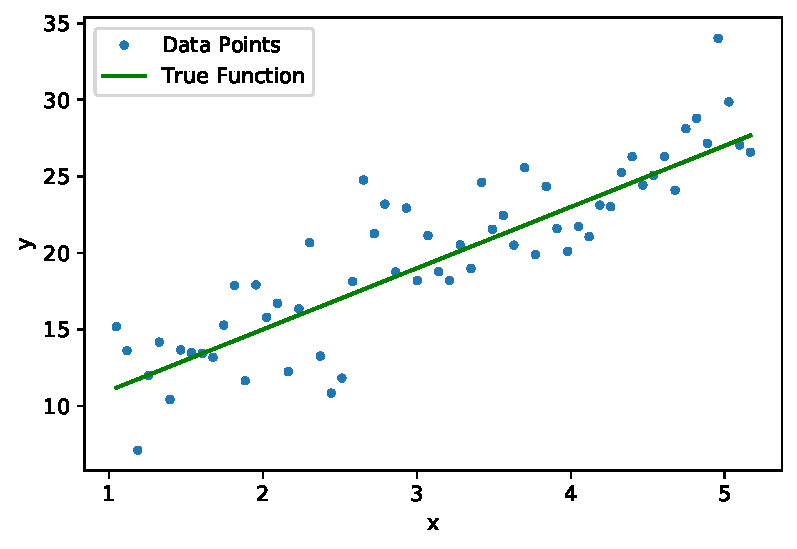
\includegraphics[scale = 0.75]{../assets/lasso/figures/true_function.pdf}
    \caption{y = 4x + 7}
    \label{fig:my_label}
\end{figure}{}

\end{frame}

\begin{frame}{Geometric Interpretation}
\begin{figure}
    \centering
    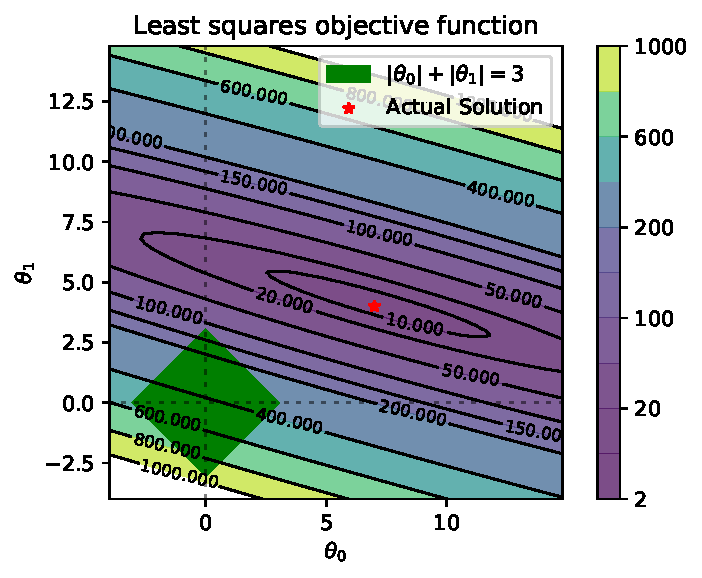
\includegraphics[scale = 0.75]{../assets/lasso/figures/lasso_base_contour.pdf}
    \caption{Lasso regression}
    \label{fig:my_label}
\end{figure}

\end{frame}

\begin{frame}{Effect of $\mu$ - Regularization of Parameters}
\vspace{0.4cm}
\begin{figure}

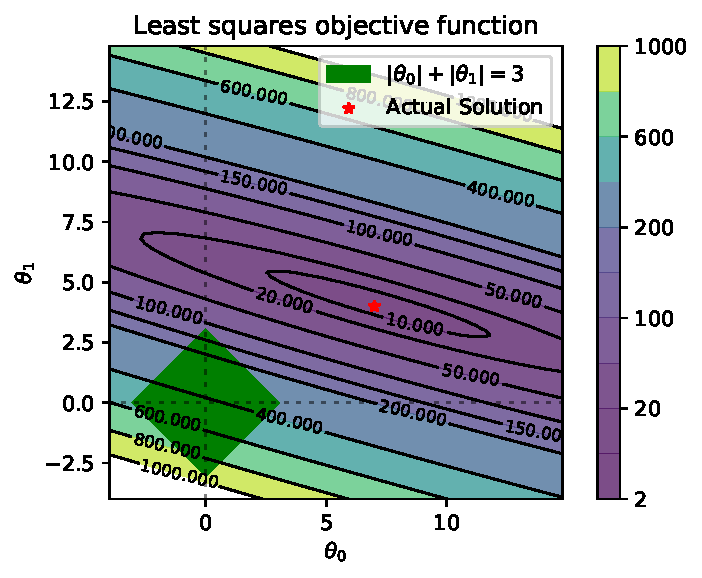
\includegraphics[width=0.9\linewidth]{../assets/lasso/figures/lasso_base_contour.pdf}
\caption{$\mu = 1.0$\\(on the \emph{Sample Dataset})}
\end{figure}
\end{frame}

\begin{frame}{Effect of $\mu$ - Regularization of Parameters}
\vspace{0.4cm}
\begin{figure}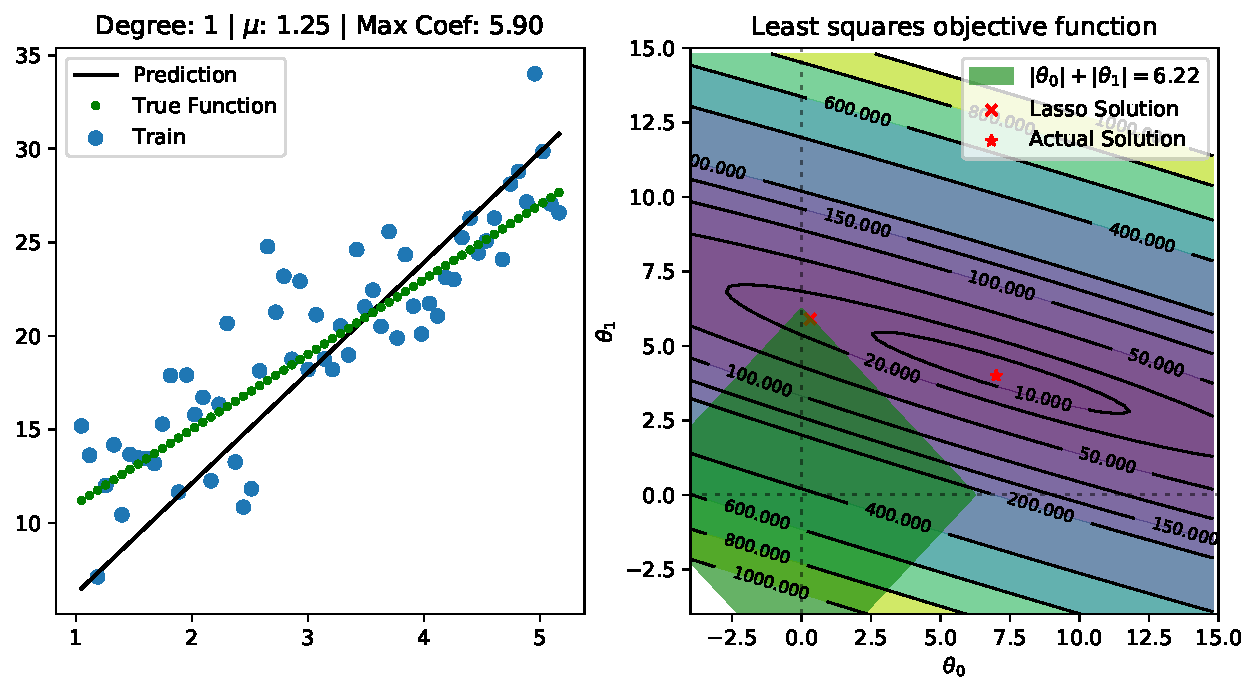
\includegraphics[width=0.9\linewidth]{../assets/lasso/figures/lasso_1.25.pdf}\caption{$\mu = 1.25$\\(on the \emph{Sample Dataset})}
\end{figure}
\end{frame}

\begin{frame}{Effect of $\mu$ - Regularization of Parameters}
\vspace{0.4cm}
\begin{figure}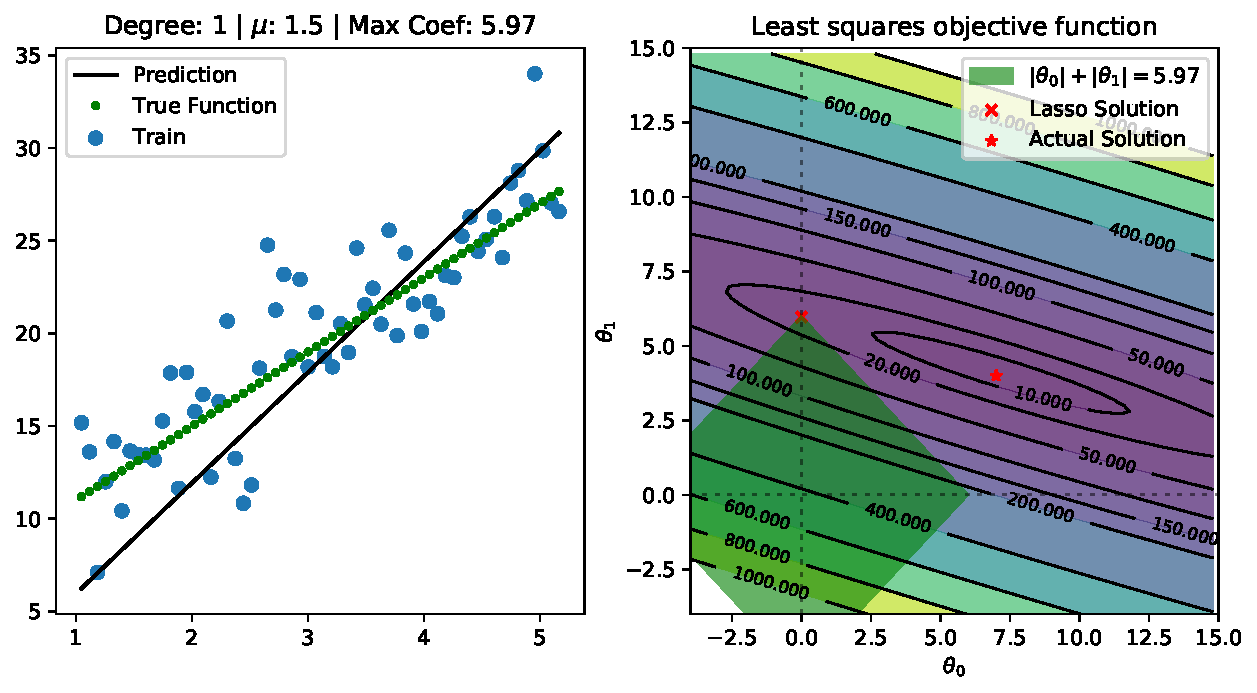
\includegraphics[width=0.9\linewidth]{../assets/lasso/figures/lasso_1.5.pdf}\caption{$\mu = 1.5$\\(on the \emph{Sample Dataset})}
\end{figure}
\end{frame}

\begin{frame}{Effect of $\mu$ - Regularization of Parameters}
\vspace{0.4cm}
\begin{figure}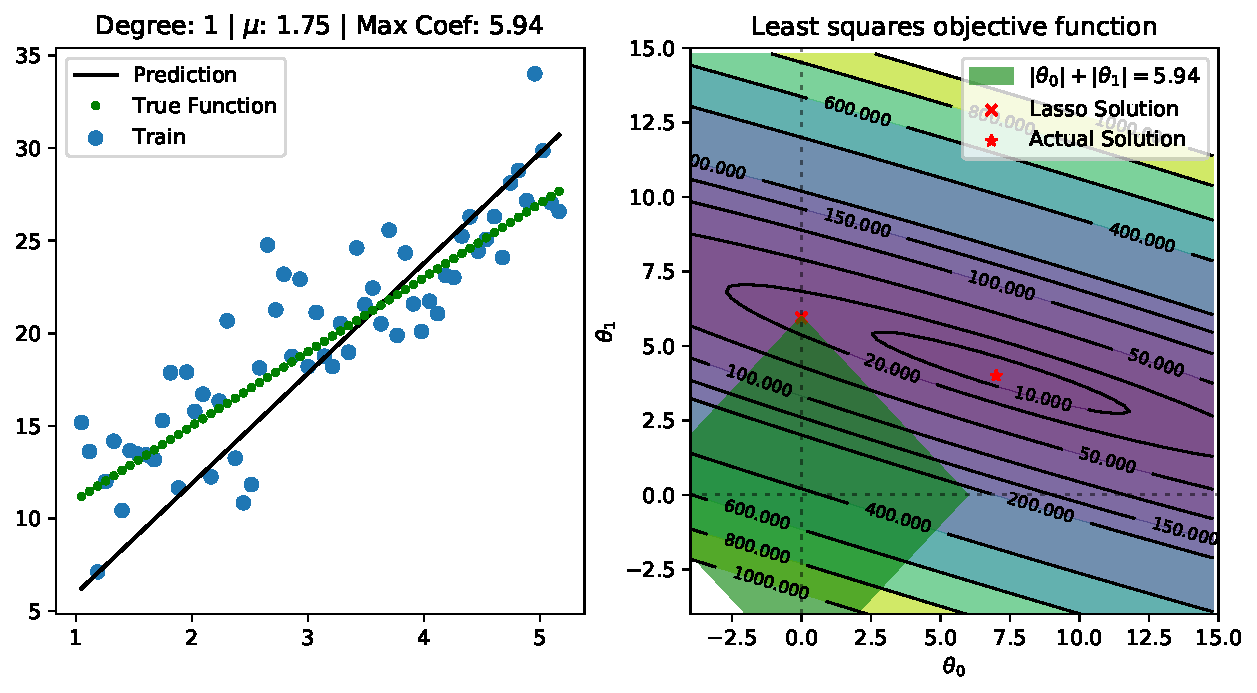
\includegraphics[width=0.9\linewidth]{../assets/lasso/figures/lasso_1.75.pdf}\caption{$\mu = 1.75$\\(on the \emph{Sample Dataset})}
\end{figure}
\end{frame}


\begin{frame}{Effect of $\mu$ - Regularization of Parameters}
\vspace{0.4cm}
\begin{figure}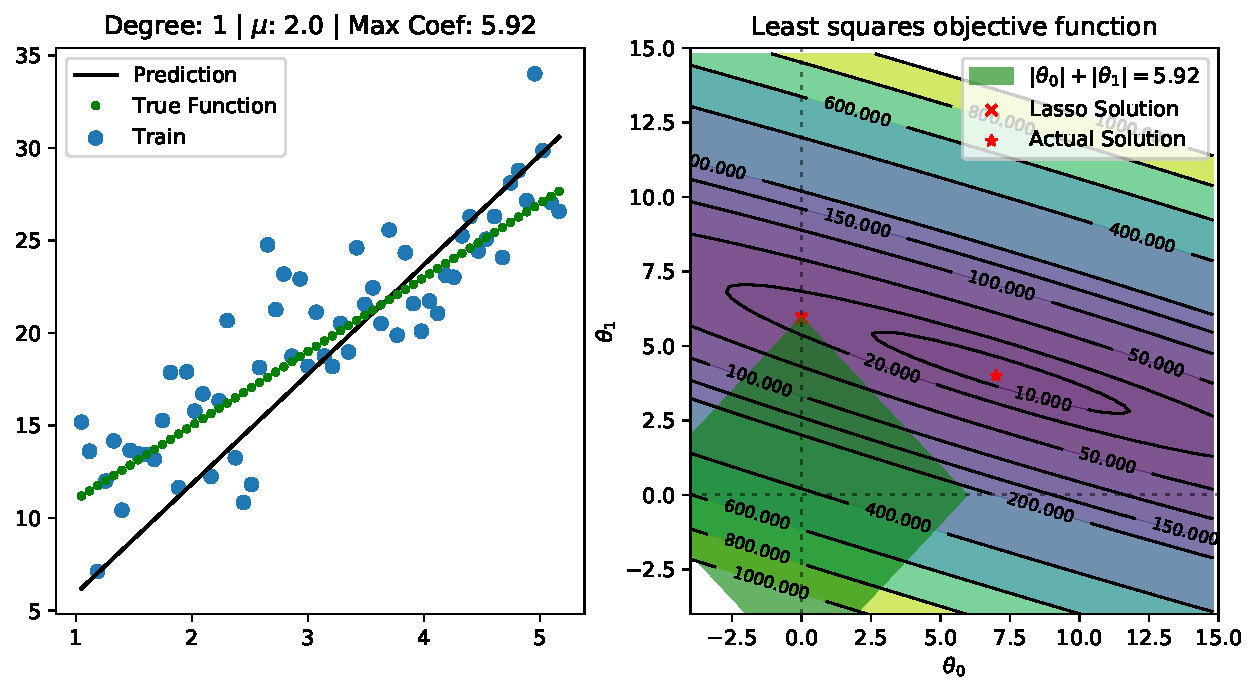
\includegraphics[width=0.9\linewidth]{../assets/lasso/figures/lasso_2.0.pdf}\caption{$\mu = 2.0$\\(on the \emph{Sample Dataset})}
\end{figure}
\end{frame}

%{
%	\setbeamercolor{background canvas}{bg=}
%	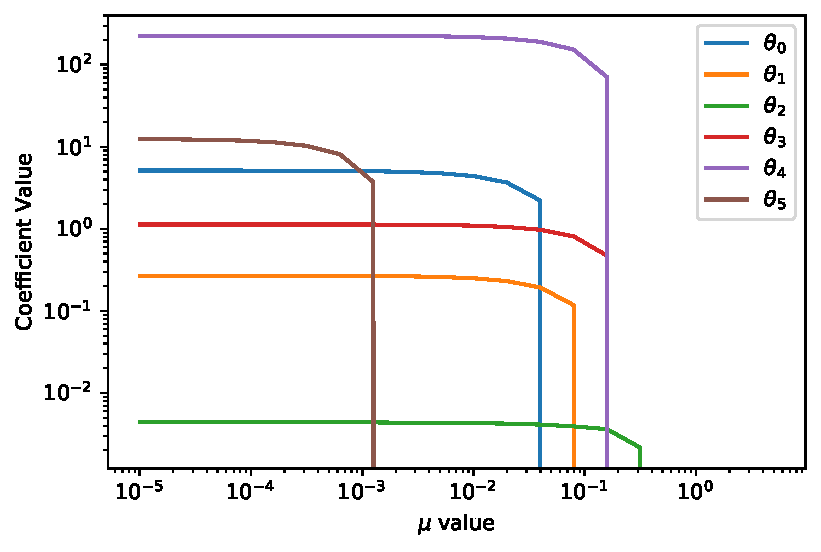
\includepdf[page=-]{lasso-sparse.pdf}
%}


%\begin{frame}{Why Lasso Gives Sparse solution}
%\begin{figure}
%    \centering
%    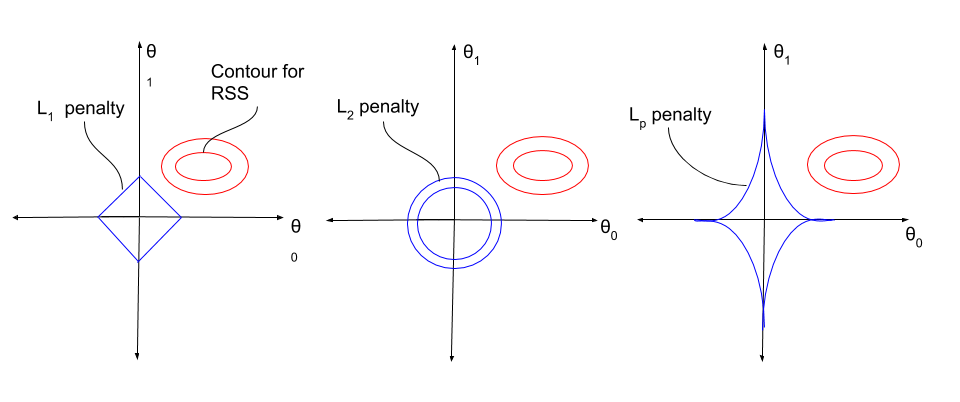
\includegraphics[scale = 0.4]{Lasso/lasso_2.png}
%    \label{fig:my_label}
%\end{figure}
%\begin{itemize}
%\small{
%    \item Pointedness of $L_{p}$ norm 
%    \item  Probability of Intersecting an axis increases.
%    \item Sparsity increases. 
%    \item Solving difficulty also increases
%    }
%\end{itemize}
%
%\end{frame}
%
%\begin{frame}{Interpretation : II}
%\begin{figure}
%    \centering
%    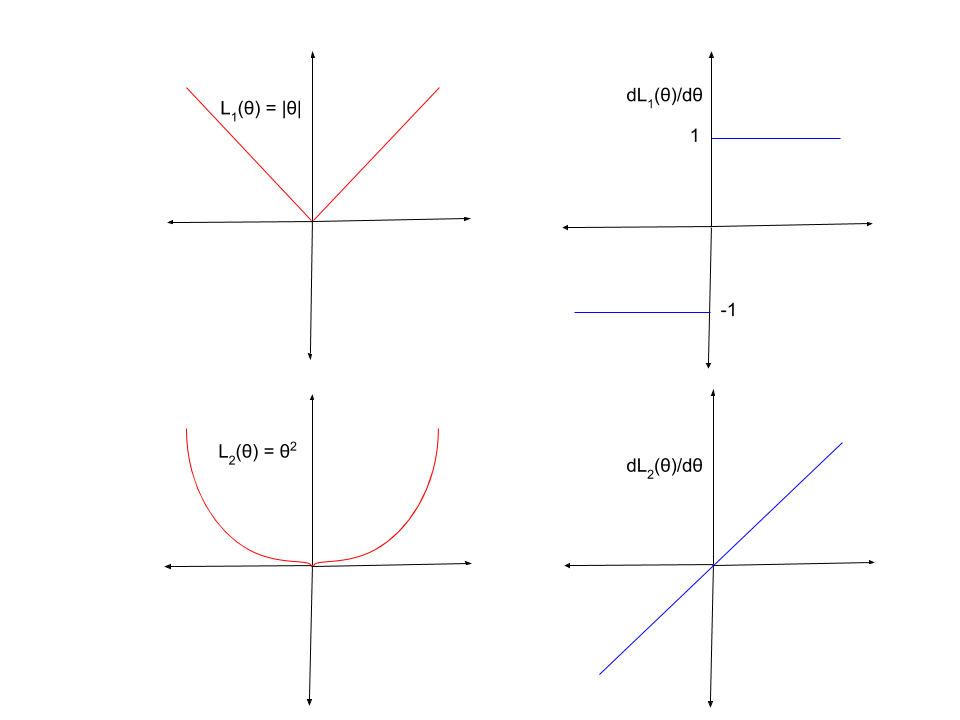
\includegraphics[scale = 0.3]{Lasso/lasso_3.png}
%    \label{fig:my_label}
%\end{figure}
%
%\end{frame}
%
%
%
%\begin{frame}{Gradient Descent}
%
%
%\foreach \x in {0,1,2,3,4} 
%{%
%\includegraphics<\x>[scale=0.75]{Lasso/GD_iteration_\x.pdf}
%%    
%}
%
%
%\end{frame}

\begin{frame}{Regularization path of lasso regression}
\begin{figure}
    \centering
    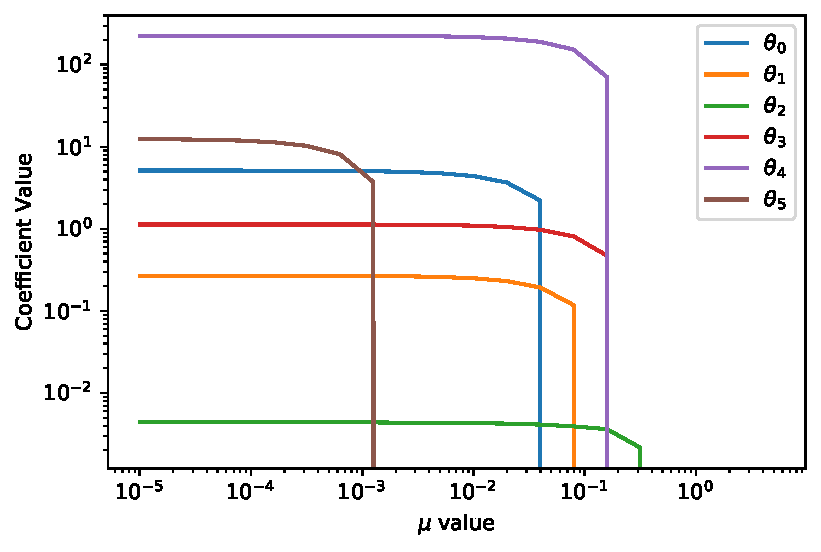
\includegraphics[scale = 0.5]{../assets/lasso/figures/lasso_reg.pdf}
    \caption{Regularization path of $\theta_{i}$}
    \label{fig:my_label}
\end{figure}

\end{frame}


\begin{frame}{LASSO and feature selection}
\begin{itemize}[<+->]
	\item LASSO inherently does feature selection!
	\item Sets coefficients of ``less important'' features to zero.
	\item Sparse and memory efficient and often more interpretable models.
\end{itemize}
\end{frame}

\begin{frame}{Subgradient }
\begin{itemize}
	
	
	\item Generalises gradient to convex but non-differentiable problems
	\item Examples:
	\begin{itemize}
		\item $f(x) = |x|$
	\end{itemize}
	
\end{itemize}
\end{frame}

\begin{frame}{Task at hand}
\begin{itemize}

\item TASK: find derivative of $f(x)$ at $x = x_0$
\end{itemize}
\begin{figure}
\centering
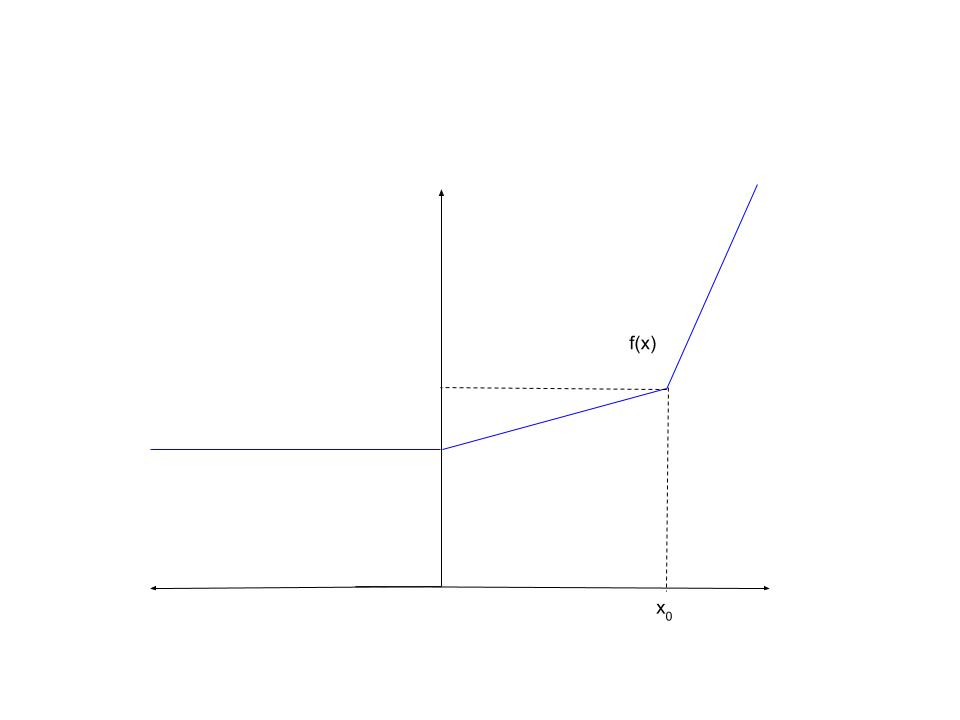
\includegraphics[scale = 0.25]{../assets/lasso/diagrams/subgradient_1.jpg}

\label{fig:Non-differentiable function}
\end{figure}


\end{frame}

\begin{frame}{Solution}

\begin{itemize}
\item Construct a differentiable $g(x)$ 
\begin{itemize}
\item Intersecting $f(x)$ at $x = x_0$
\item Below or on $f(x)$ for all x
\end{itemize}
\end{itemize}
\begin{figure}
\centering
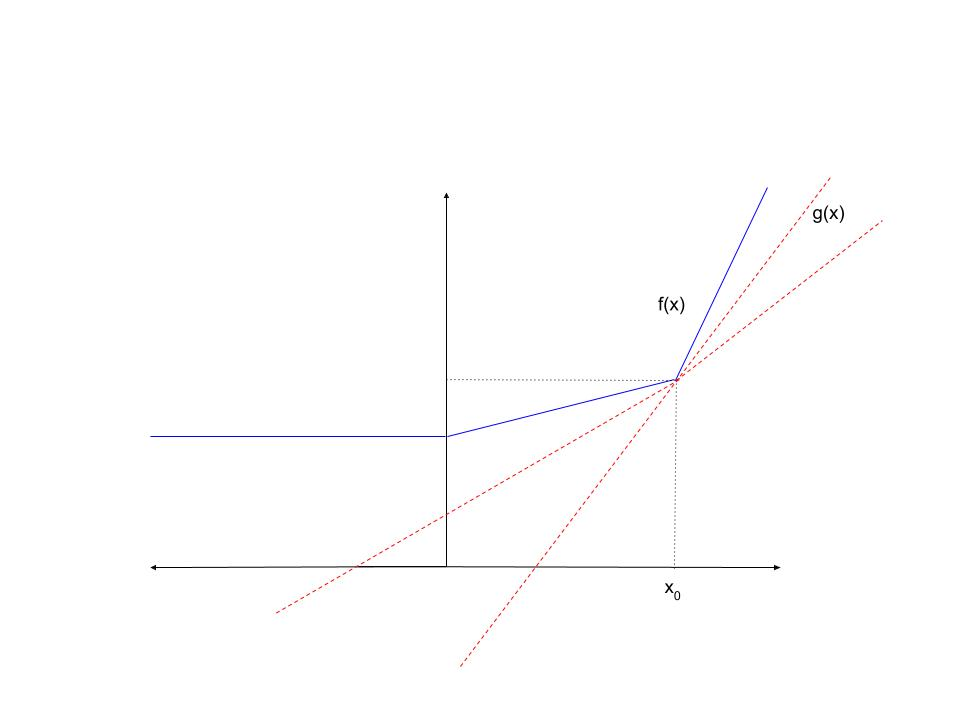
\includegraphics[scale = 0.25]{../assets/lasso/diagrams/subgradient_2.jpg}
\label{fig:my_label}
\end{figure}
\end{frame}

\begin{frame}{Solution}

\begin{itemize}
\item Compute slope of $g(x)$ at $x = x_0$
\end{itemize}
\begin{figure}
\centering
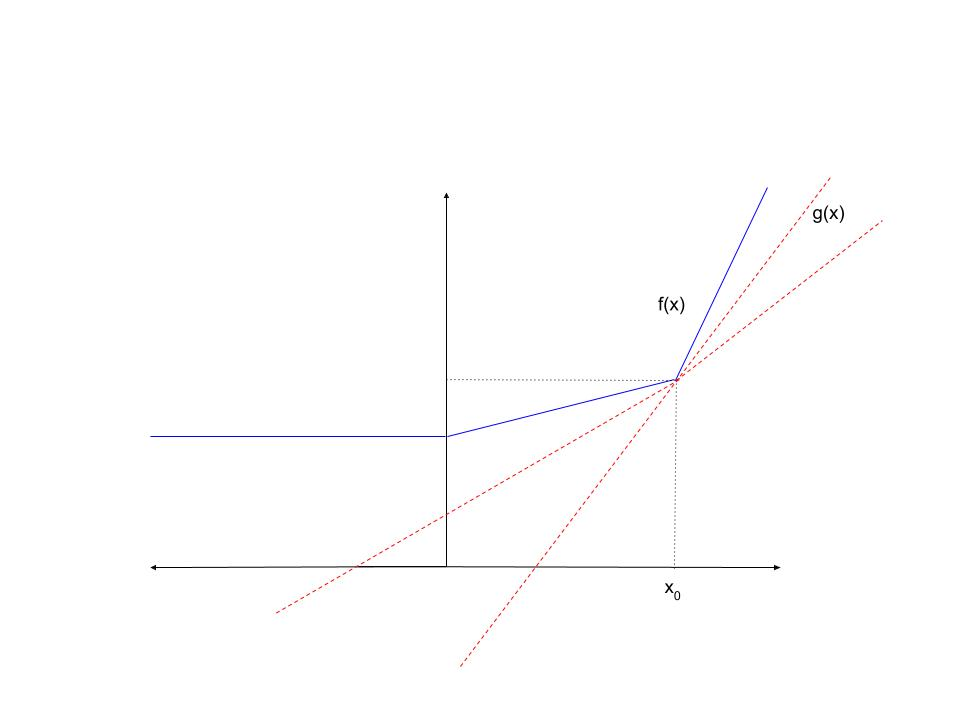
\includegraphics[scale = 0.25]{../assets/lasso/diagrams/subgradient_2.jpg}

\label{fig:my_label}
\end{figure}
\end{frame}

\begin{frame}{Another Example: $f(x) = |x|$}

\begin{itemize}
\item Subgradient of $f(x)$ belongs to $[-1, 1]$
\end{itemize}
\begin{figure}
\centering
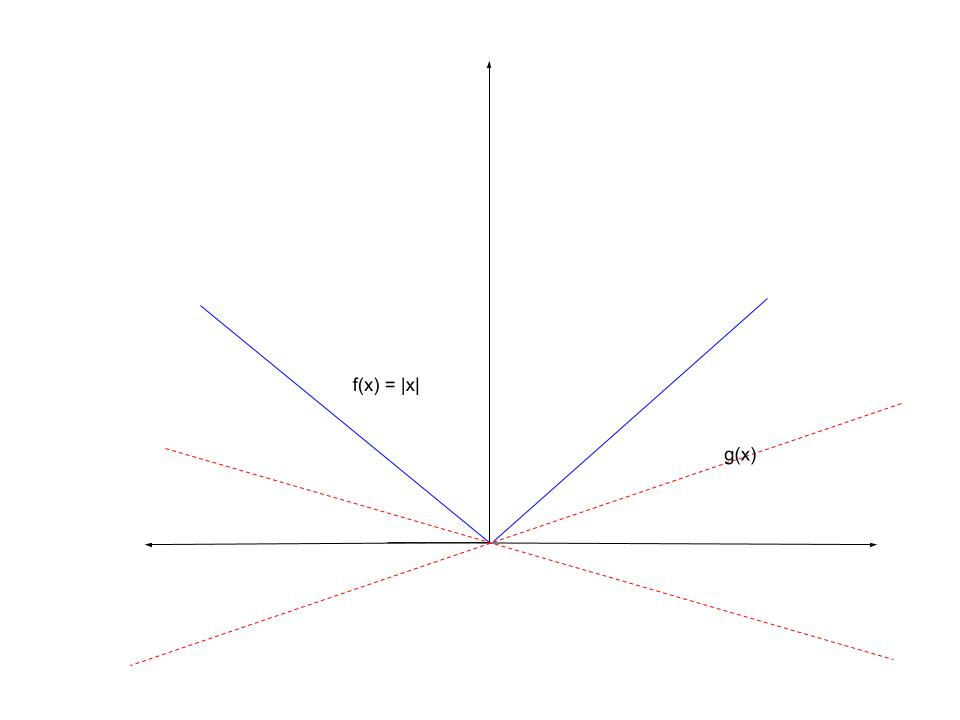
\includegraphics[scale = 0.25]{../assets/lasso/diagrams/subgradient_3.jpg}
\label{fig:my_label}
\end{figure}
\end{frame}

\begin{frame}{Coordinate Descent}
\begin{itemize}[<+->]
	\item Another optimisation method (akin to gradient descent)
	\item Objective: $\min_{\vtheta} f(\vtheta)$
	\item Key idea: Sometimes difficult to find minimum for all coordinates
	\item ..., but, easy for each coordinate
	\item turns into a one-dimensional optimisation problem
\end{itemize}
\end{frame}

%{
%\setbeamercolor{background canvas}{bg=}
%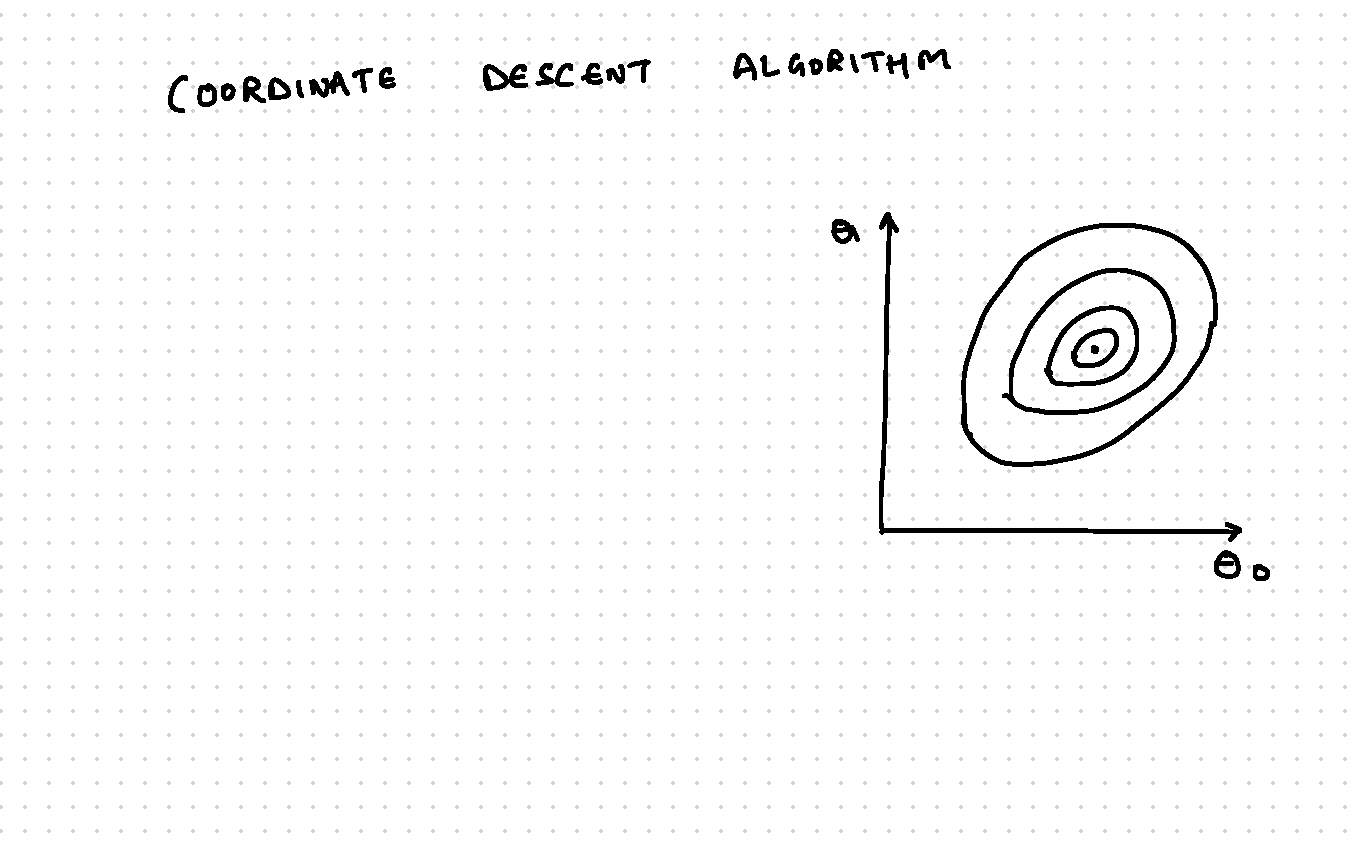
\includepdf[page=-]{coordinate-vis.pdf}
%}


\begin{frame}{Coordinate Descent}
\begin{itemize}[<+->]
\item Picking next coordinate: \pause random, round-robin
\item No step-size to choose!
\item Converges for Lasso objective
\end{itemize}
\end{frame}




\begin{frame}{Coordinate Descent : Example}
Learn $y = \theta_0 + \theta_1 x$ on following dataset, using coordinate descent where initially $(\theta_0, \theta_1) = (2,3)$  for 2 iterations. 
\begin{table}[]
\centering
\label{tab:my-table}
\begin{tabular}{|c|c|}
\hline
\textbf{x} & \textbf{y} \\ \hline
1 & 1 \\ \hline
2 & 2 \\ \hline
3 & 3 \\ \hline
\end{tabular}
\end{table}
\end{frame}



\begin{frame}{Coordinate Descent : Example}
Our predictor, $\hat{y} = \theta_0 + \theta_1x$\\
\vspace{1cm}
Error for $i^{th}$ datapoint, $\epsilon_i = y_i - \hat{y_i}$\\
$\epsilon_1 = 1 - \theta_0 - \theta_1$ \\
$\epsilon_2 = 2 - \theta_0 - 2\theta_1$ \\
$\epsilon_3 = 3 - \theta_0 - 3\theta_1$ \\

\vspace{1cm}
$\MSE = \frac{\epsilon_1^2 + \epsilon_2^2 + \epsilon_3^2}{3} = \frac{14 + 3\theta_0^2 + 14\theta_1^2 -12\theta_0 - 28\theta_1 + 12\theta_0\theta_1}{3}$\\
\end{frame}





\begin{frame}{Iteration 0}

MSE = $\frac{1}{3}(14+3\theta_{0}^{2}+14\theta_{1}^{2}-12\theta_{0}-28\theta_{1}+12\theta_{0}\theta_{1})$\\

\begin{columns}
\begin{column}{0.6\textwidth}
\begin{adjustbox}{max totalsize={\textwidth},center}

\begin{tikzpicture}
\begin{axis}[colorbar,xlabel=$\theta_0$, ylabel=$\theta_1$, zlabel=$\mathrm{Cost Function}$,title={Surface Plot}]
\addplot3[
surf,opacity=0.1,
]
{(14 + 3*x^2 +14*y^2 -12*x - 28*y + 12*x*y)/3};
\addplot[only marks, mark=*]
coordinates{ % plot 1 data set
( 2 , 3 )
}; 
\end{axis}
\end{tikzpicture}
\end{adjustbox}

\end{column}
\begin{column}{0.5\textwidth}
\begin{adjustbox}{max totalsize={\textwidth},center}
\begin{tikzpicture}
\begin{axis}
[
title={Contour plot, view from top},
view={0}{90},
xlabel=$\theta_0$,
ylabel=$\theta_1$,
axis x line*=bottom,
axis y line*=left,
xtick align=outside,
ytick align=outside,
unit vector ratio*=1 1 1,
]
\addplot3[
contour gnuplot={number=25,}
]
{(14 + 3*x^2 +14*y^2 -12*x - 28*y + 12*x*y)/3};
\addplot[only marks, mark=*]
coordinates{ % plot 1 data set
( 2 , 3 )
};


\end{axis}
\end{tikzpicture}
\end{adjustbox}
\end{column}
\end{columns}




\end{frame}

\begin{frame}{Coordinate Descent : Example}
\textbf{Iteration 1}\\
\vspace{0.5cm}
INIT: $\theta_{0} = 2$ and  $\theta_{1}  = 3$\\

\vspace{0.5cm}
$\theta_1 = 3$ optimize for $\theta_{0}$\\ 
\only<2->{
\vspace{0.5cm}
$\frac{\partial \MSE}{\partial \theta_{0}} = 6\theta_0 + 24 = 0$\\
\vspace{0.5cm}
$\theta_0 = -4$


}


\end{frame}


\begin{frame}{Iteration 1}

MSE = $\frac{1}{3}(14+3\theta_{0}^{2}+14\theta_{1}^{2}-12\theta_{0}-28\theta_{1}+12\theta_{0}\theta_{1})$\\

\begin{columns}
\begin{column}{0.6\textwidth}
\begin{adjustbox}{max totalsize={\textwidth},center}

\begin{tikzpicture}
\begin{axis}[colorbar,xlabel=$\theta_0$, ylabel=$\theta_1$, zlabel=$\mathrm{Cost Function}$,title={Surface Plot}]
\addplot3[
surf,opacity=0.1,
]
{(14 + 3*x^2 +14*y^2 -12*x - 28*y + 12*x*y)/3};
\addplot[only marks, mark=*]
coordinates{ % plot 1 data set
( -4 , 3 )
}; 

\end{axis}
\end{tikzpicture}
\end{adjustbox}

\end{column}
\begin{column}{0.5\textwidth}
\begin{adjustbox}{max totalsize={\textwidth},center}
\begin{tikzpicture}
\begin{axis}
[
title={Contour plot, view from top},
view={0}{90},
xlabel=$\theta_0$,
ylabel=$\theta_1$,
axis x line*=bottom,
axis y line*=left,
xtick align=outside,
ytick align=outside,
unit vector ratio*=1 1 1,
]
\addplot3[
contour gnuplot={number=25,}
]
{(14 + 3*x^2 +14*y^2 -12*x - 28*y + 12*x*y)/3};
\draw [->] (axis cs: 2,3) -- (axis cs:-4,3);
\end{axis}
\end{tikzpicture}
\end{adjustbox}
\end{column}
\end{columns}


\end{frame}

\begin{frame}{Coordinate Descent : Example}
\textbf{Iteration 2}\\
\vspace{0.5cm}
INIT: $\theta_{0} = -4$ and  $\theta_{1}  = 3$\\

\vspace{0.5cm}
$\theta_0 = -4$ optimize for $\theta_{1}$\\ 
\only<2->{
\vspace{0.5cm}
$\theta_1 = 2.7$
}


\end{frame}


\begin{frame}{Iteration 2}

MSE = $\frac{1}{3}(14+3\theta_{0}^{2}+14\theta_{1}^{2}-12\theta_{0}-28\theta_{1}+12\theta_{0}\theta_{1})$\\

\begin{columns}
\begin{column}{0.6\textwidth}
\begin{adjustbox}{max totalsize={\textwidth},center}

\begin{tikzpicture}
\begin{axis}[colorbar,xlabel=$\theta_0$, ylabel=$\theta_1$, zlabel=$\mathrm{Cost Function}$,title={Surface Plot}]
\addplot3[
surf,opacity=0.1,
]
{(14 + 3*x^2 +14*y^2 -12*x - 28*y + 12*x*y)/3};
\addplot[only marks, mark=*]
coordinates{ % plot 1 data set
( -4 , 2.7 )
}; 

\end{axis}
\end{tikzpicture}
\end{adjustbox}

\end{column}
\begin{column}{0.5\textwidth}
\begin{adjustbox}{max totalsize={\textwidth},center}
\begin{tikzpicture}
\begin{axis}
[
title={Contour plot, view from top},
view={0}{90},
xlabel=$\theta_0$,
ylabel=$\theta_1$,
axis x line*=bottom,
axis y line*=left,
xtick align=outside,
ytick align=outside,
unit vector ratio*=1 1 1,
]
\addplot3[
contour gnuplot={number=25,}
]
{(14 + 3*x^2 +14*y^2 -12*x - 28*y + 12*x*y)/3};
\draw [->] (axis cs: 2,3) -- (axis cs:-4,3);
\draw [->] (axis cs: -4,3) -- (axis cs:-4,2.7);
\end{axis}
\end{tikzpicture}
\end{adjustbox}
\end{column}
\end{columns}


\end{frame}

\begin{frame}{Coordinate Descent : Example}
\textbf{Iteration 3}\\
\vspace{0.5cm}
INIT: $\theta_{0} = -4$ and $\theta_{1}  = 2.7$\\

\vspace{0.5cm}
$\theta_1 = 2.7$ optimize for $\theta_{0}$\\ 
\only<2->{
\vspace{0.5cm}
$\theta_0 = -3.4$
}


\end{frame}

\begin{frame}{Iteration 3}

MSE = $\frac{1}{3}(14+3\theta_{0}^{2}+14\theta_{1}^{2}-12\theta_{0}-28\theta_{1}+12\theta_{0}\theta_{1})$\\

\begin{columns}
\begin{column}{0.6\textwidth}
\begin{adjustbox}{max totalsize={\textwidth},center}

\begin{tikzpicture}
\begin{axis}[colorbar,xlabel=$\theta_0$, ylabel=$\theta_1$, zlabel=$\mathrm{Cost Function}$,title={Surface Plot}]
\addplot3[
surf,opacity=0.1,
]
{(14 + 3*x^2 +14*y^2 -12*x - 28*y + 12*x*y)/3};
\addplot[only marks, mark=*]
coordinates{ % plot 1 data set
( -3.4 , 2.7 )
}; 
\end{axis}
\end{tikzpicture}
\end{adjustbox}

\end{column}
\begin{column}{0.5\textwidth}
\begin{adjustbox}{max totalsize={\textwidth},center}
\begin{tikzpicture}
\begin{axis}
[
title={Contour plot, view from top},
view={0}{90},
xlabel=$\theta_0$,
ylabel=$\theta_1$,
axis x line*=bottom,
axis y line*=left,
xtick align=outside,
ytick align=outside,
unit vector ratio*=1 1 1,
]
\addplot3[
contour gnuplot={number=25,}
]
{(14 + 3*x^2 +14*y^2 -12*x - 28*y + 12*x*y)/3};
\draw [->] (axis cs: 2,3) -- (axis cs:-4,3);
\draw [->] (axis cs: -4,3) -- (axis cs:-4,2.7);
\draw [->] (axis cs: -4,2.7) -- (axis cs:-3.4,2.7);
\end{axis}
\end{tikzpicture}
\end{adjustbox}
\end{column}
\end{columns}


\end{frame}


%{
%\setbeamercolor{background canvas}{bg=}
%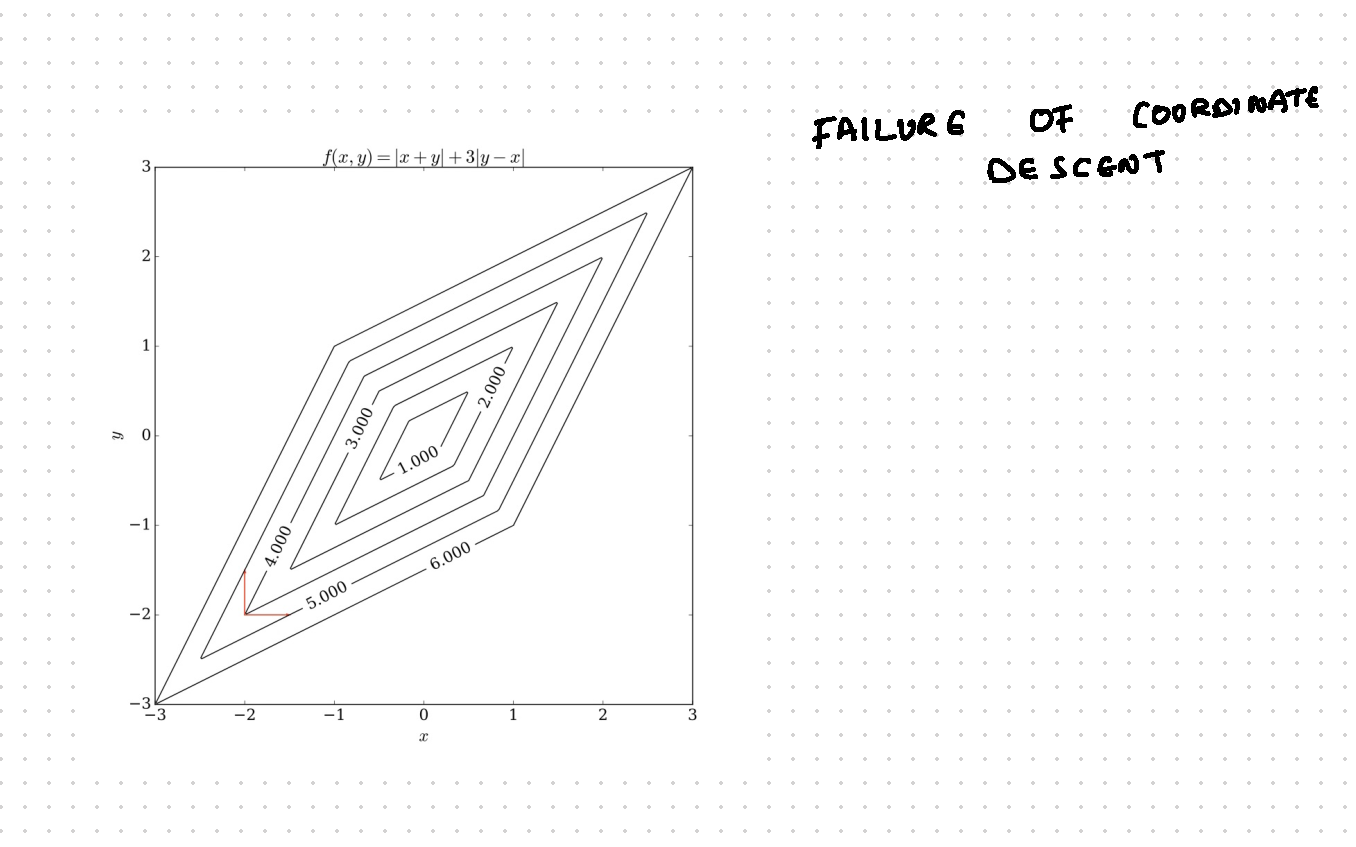
\includepdf[page=-]{coordinate-descent-fail.pdf}
%}


\begin{frame}{Coordinate Descent for Unregularised Regression}

\begin{itemize}[<+->]
	
	
	
	
	
	\item Express error as a difference of $y_{i}$ and $\hat{y_{i}}$
	\begin{align}
	\hat{y_i} &= \sum_{j=0}^{d} \theta_{j}x^{j}_{i} = \theta_{0}x_{i}^{0} + \theta_{1}x_{i}^{1} +\theta_{2}x_{i}^{2} + \ldots + \theta_{d}x_{i}^{d}  \\
	\epsilon_{i} &= y_{i} - \hat{y_{i}}\\
	&= y_{i} - \theta_{0}x_{i}^{0} + \theta_{1}x_{i}^{1} + \ldots + \theta_{d}x_{i}^{d}\\
	&= y_{i} - \sum_{j=0}^{d} \theta_{j}x_{i}^{j}
	\end{align}
	
	
	
\end{itemize}


\end{frame}



\begin{frame}{Coordinate Descent for Unregularised regression}

\begin{align*}
\sum_{i=1}^{n}  \epsilon^{2}=\RSS &=\sum_{i=1}^{n}\left(y_{i}-\left(\theta_{0}x_{i}^{0}+\ldots \quad \theta_{j} x_{i}^{j}+\theta_{d} x_{i}^{d}\right)\right)^{2}\\
\end{align*}
\end{frame}

\begin{frame}{Coordinate Descent for Unregularised regression}

\begin{align*}
\sum_{i=1}^{n}  \epsilon^{2}=\RSS &=\sum_{i=1}^{n}\left(y_{i}-\left(\theta_{0}x_{i}^{0}+\ldots \quad \theta_{j} x_{i}^{j}+\theta_{d} x_{i}^{d}\right)\right)^{2}\\
\frac{\partial \RSS\left(\theta_{j}\right)}{\partial \theta_{j}}&= 2 \sum_{i=1}^{n}\left(y_{i}-\left(\theta_{0}x_{i}^{0}+\ldots \quad \theta_{j} x_{i}^{j}+\ldots \right)\right)\left(-x_{i}^{j}\right)\\
\end{align*}
\end{frame}

\begin{frame}{Coordinate Descent for Unregularised regression}

\begin{align*}
\sum_{i=1}^{n}  \epsilon^{2}=\RSS &=\sum_{i=1}^{n}\left(y_{i}-\left(\theta_{0}x_{i}^{0}+\ldots \quad \theta_{j} x_{i}^{j}+\theta_{d} x_{i}^{d}\right)\right)^{2}\\
\frac{\partial \RSS\left(\theta_{j}\right)}{\partial \theta_{j}}&= 2 \sum_{i=1}^{n}\left(y_{i}-\left(\theta_{0}x_{i}^{0}+\ldots \quad \theta_{j} x_{i}^{j}+\ldots \right)\right)\left(-x_{i}^{j}\right)\\
&=2\sum_{i=1}^{n}\left(y_{i}-\left(\theta_{0} x_{i}^{0}+\ldots + \theta_{d} x_{i}^{d}\right)\right)\left(-x_{i}^{j}\right)+2 \sum_{i=1}^{n} \theta_{j}(x_{i}^j)^2\\
\end{align*}
\pause where: $$\hat{y_{i}}^{(-j)} = \theta_{0} x_{i}^{0}+\ldots + \theta_{d} x_{i}^{d}$$ is $\hat{y}_{i}$ without $\theta_{j}$
\end{frame}

\begin{frame}{Coordinate Descent for Unregularised regression}

\begin{align*}
Set \frac{\partial \RSS\left(\theta_{j}\right)}{\partial \theta_{j}}&= 0\\
\theta_{j}&=\sum_{i=1}^{n} \frac{\left(y_{i}-\left(\theta_{0} x_{i}^{0}+\ldots + \ldots + \theta_{d}
x_{i}^{d}\right)\right)\left(x_{i}^{j}\right)}{\left(x_{i}^{j}\right)^{2}}= \frac{\rho_{j}}{z_{j}}\\
\rho_{j} &=\sum_{i=1}^{n} x_{i}^{j}\left(y_{i}-{\hat{y}_{i}^{(-j)}})\right)\\
z_{j}&=\sum_{i=1}^{n}\left(x_{i}^{j}\right)^{2}
\end{align*}
$z_{j}$ is the squared of $\ell_2$ norm of the $j^{th}$ feature
\end{frame}

%{
%\setbeamercolor{background canvas}{bg=}
%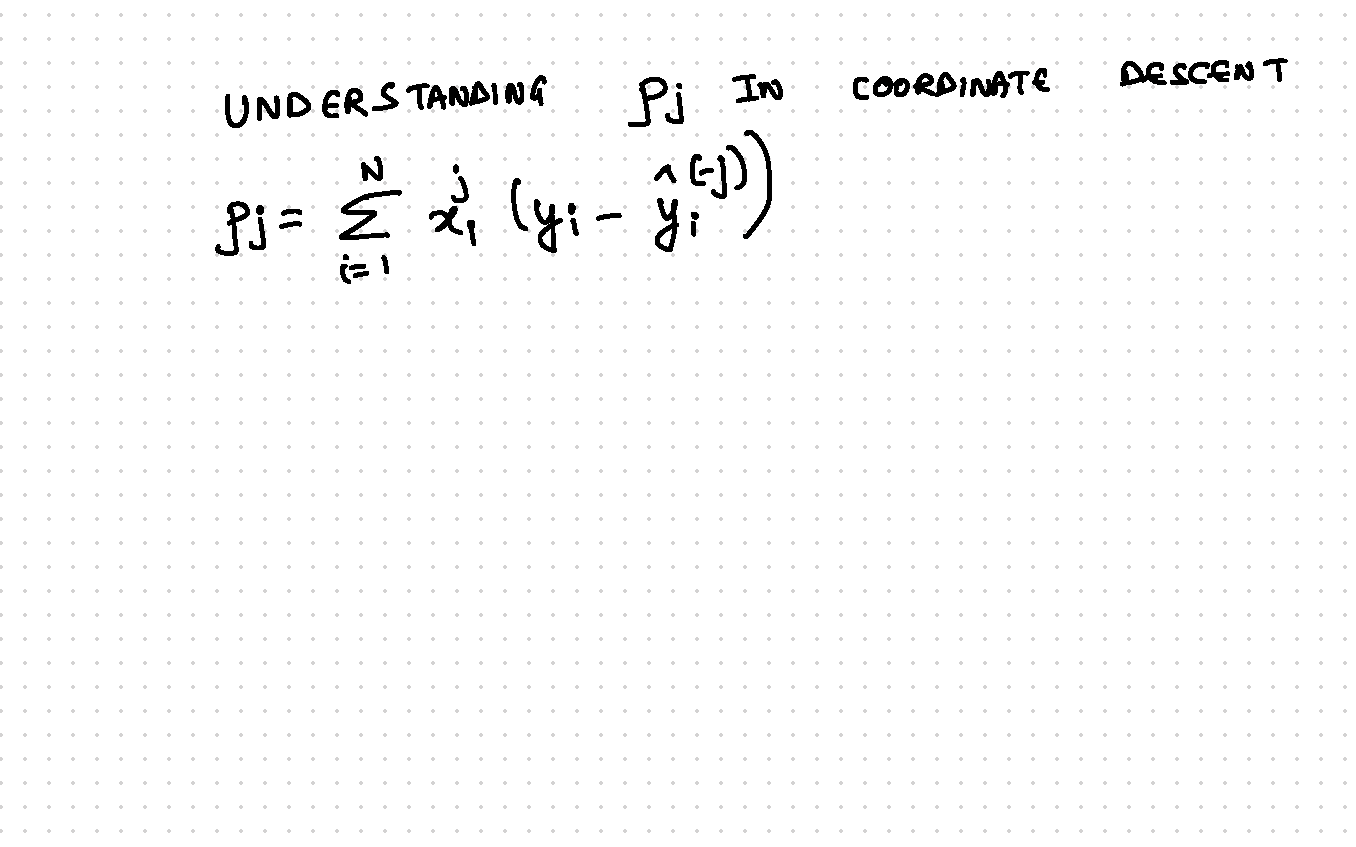
\includepdf[page=-]{coordinate-rho.pdf}
%}




\begin{frame}{Coordinate Descent for Lasso Regression}
\[
\text{Minimise} \underbrace{\sum_{i=1}^{n} \epsilon^{2} + \delta^{2}\left\{\left|\theta_{0}\right|+\left|\theta_{1}\right|+\ldots\left|\theta_{j}\right|+\ldots |\theta_{d}|\right\}}_{\text{LASSO OBJECTIVE}}
\]
\begin{align*}
\frac{\partial}{\partial \theta_{j}}(& \text {LASSO OBJECTIVE})=-2 \rho_{j}+2 \theta_{j} z_{j}+\delta^{2}{\frac{\partial}{\partial \theta_{j}}}\left|\theta_{j}\right|\\[18pt]
&\frac{\partial}{\partial \theta_{j}}\left|\theta_{j}\right|=\left\{\begin{array}{cc}
{1} & {\theta_{j}>0} \\
{[-1,1]} & {\theta_{j}=0} \\
{-1} & {\theta_{j}<0}
\end{array}\right.
\end{align*}
\end{frame}

\begin{frame}{Coordinate Descent for Lasso Regression}
\begin{itemize}[<+->]
\item \textbf{Case 1: $\theta_{j}>0$}
\begin{align*}
\-2\rho_j+2\theta_j z_j+\delta^{2}  = 0\\
\theta_j = \frac{\rho_j - \frac{\delta^{2}}{2}}{z_{j}}\\
\rho_{j}>\frac{\delta^{2}}{2} \Rightarrow  \theta_{j} = \frac{\rho_j - \frac{\delta^{2}}{2}}{z_{j}}
\end{align*}

\item \textbf{Case 2: $\theta_{j}<0$}
\begin{equation}
\rho_{j} < \frac{\delta^{2}}{2} \Rightarrow \theta_{j} = \frac{\rho_{j}+\delta^{2} / 2}{z_{j}}
\end{equation}
\end{itemize}

\end{frame}

\begin{frame}{Coordinate Descent for Lasso Regression}
\begin{itemize}
\item \textbf{Case 3: $\theta_{j} = 0$}
\begin{align*}
\frac{\partial}{\partial \theta_{j}}(\text {LASSO OBJECTIVE})&=-2 \rho_{j}+2\theta_{j} z_{j}+ \delta^{2}\underbrace{{\frac{\partial}{\partial \theta_{j}}}\left|\theta_{j}\right|}_{\text{[-1,1]}}\\
&\in \underbrace{[-2\rho_{j} - \delta^{2}, -2\rho_{j} + \delta^{2}]}_{\text{$\{0\}$ lies in this range}}\\
\end{align*}
\begin{align*}
-2\rho_{j} - \delta^{2} \leq 0 \text{ and }& -2\rho_{j} - \delta^{2} \leq 0\\
-\frac{\delta^{2}}{2} \leq \rho_j \leq \frac{\delta^{2}}{2}  \Rightarrow & \hspace{2mm} \theta_{j}=0
\end{align*}

\end{itemize}

\end{frame}
\begin{frame}{Summary of Lasso Regression}
\begin{equation}
\theta_{j} =\left[\begin{array}{ccc}
{\frac{\rho_{j} + \frac{\delta^{2}}{2}}{z_{j}}} & {if}  & {\rho_{j}<-\frac{\delta^{2}}{2}} \\
{0} & {if} & {-\frac{\delta^{2}}{2} \leq \rho_{j} \leq \frac{\delta^{2}}{2}} \\
{\frac{\rho_{j} - \frac{\delta^{2}}{2}}{z_{j}}} & {i f} & {\rho_{j}>\frac{\delta^{2}}{2}}
\end{array}\right]
\end{equation}

\end{frame}

%{
%\setbeamercolor{background canvas}{bg=}
%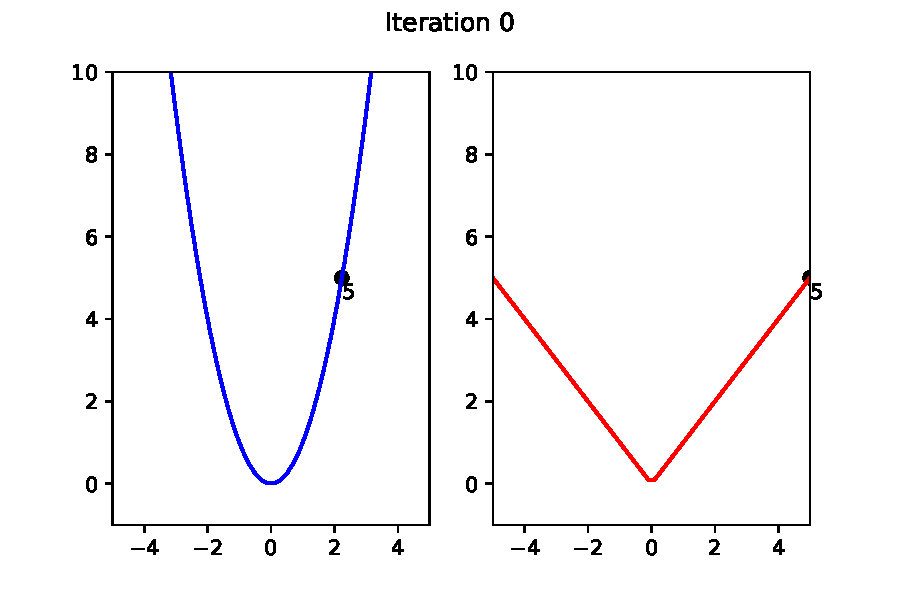
\includepdf[page=-]{coordinate-thresholding.pdf}
%}


\end{document}
